\documentclass[conference]{Template/IEEEtran}
\IEEEoverridecommandlockouts
\usepackage{cite}
\usepackage{amsmath,amssymb,amsfonts}
\usepackage{algorithmic}
\usepackage{graphicx}
\usepackage{textcomp}
\usepackage{xcolor}
\usepackage{float}
\usepackage{subfigure}
\usepackage{steinmetz}
\usepackage [hidelinks, breaklinks=true] {hyperref} 
\usepackage{float}
\usepackage{color}
\usepackage{tikz}
\usepackage{subfigure} 
\usepackage{pdfpages}
\usepackage{fancyhdr}
\usepackage{textcomp} %para simbolo de marca registrada
\def\BibTeX{{\rm B\kern-.05em{\sc i\kern-.025em b}\kern-.08em
    T\kern-.1667em\lower.7ex\hbox{E}\kern-.125emX}}
    
   \graphicspath{Figuras/ }

%Configuración del pie de página. Se puede hacer con fancyfoot o por cada bloque de pie separado (izq, derecho y central; lo mismo para la cabecera) . Si no se deja en blanco cfoot{} el numero de pagina se pone al medio por default y pisa las letras de las otras cosas. 

\pagestyle{fancy}
%\fancyfoot[L]{}
\lfoot{\textsc{UTN,FRC. Cátedra Electrónica de Potencia - Paper N$^{\circ}$} 9541-059/20}
\cfoot{} % quitar número de página del centro
\rfoot{\thepage} % número de página a la derecha
\renewcommand{\headrulewidth}{0pt} % grosor de la línea de la cabecera
\renewcommand{\footrulewidth}{0pt} % grosor de la línea del pie

  %foot layout 
\pagestyle{fancy}
\title{Diseño de conversor Buck-Boost - SEPIC- para celdas fotovoltaicas con MPPT} 
\author{
\IEEEauthorblockN{ Matias Dogliani [72152@electronica.utn.frc.edu.ar]}
\IEEEauthorblockA{\textit{Universidad Tecnológica Nacional, Departamento de Ingeniería Electrónica} \\
\textit{Electrónica de Potencia} \\
2020} \\

}



    %Tittle and author layout 

\begin{document}
\maketitle\thispagestyle{fancy}
\begin{abstract}


    In this paper a low-cost and simple DC-DC Buck-Boost converter is designed for photo-voltaic (PV) aplicattions, for Maximum Power Point Tracking integration for variable voltage input and variable load (i.e charging a battery bank system) suitable for residencial use. 
    

\end{abstract}
\begin{resumen}
    Acá va el resumen en español \\ 
    Con varias lineas \\ 
    para probar si anda \\ 
    
\end{resumen}

\begin{IEEEkeywords}
   Dc-dc converter, MPPT, PV, Solar, buck-boost
\end{IEEEkeywords}

%Cambiar abstract. Darle enfioque domiciliaroi  

\section{Introducción}

    En los últimos años se ha presenciado el auge de las energías renovables, principalmente por el aumento de la demanda de energía a nivel mundial conjuntamente con el aumento del costo de la misma y el altamente negativo impacto ambiental del uso de la energía convencional (fósil) \cite{gallardo2014diseno}. La energía solar, perteneciente a las energías denominadas limpias, puede ser utilizada fácilmente en sistemas de energía  residenciales y/o industriales, particularmente en áreas rurales o remotas. 
    
    En las interfaces utilizadas entre las celdas fotovoltaicas y la carga domiciliaria (cargadores de baterías, luminaria DC, etc) podemos encontrar conversores de bajo costo pero así de también de una eficiencia reducida dado que el punto de operación de los paneles solares, en la mayoría de los casos, no es adecuado \cite{Chang}. Distintos tipos de conversores DC-DC son utilizados, donde cada uno presenta cierta deficiencia y o limitación en cuanto a la regulación de voltaje de entrada y salida, valor de carga, etc. Además el control de estos conversores de bajo costo se realiza con técnicas basadas en PWM. 
    
    Considerando las características de los paneles PV, el voltaje de salida de los mismos varia ampliamente de acuerdo a la temperatura ambiente, radiación solar, tiempo de sombra, y otras condiciones climáticas como así también de parámetros inherentes de los mismos como conexión de celdas, cantidad de celdas,etc. Por lo que para lograr un voltaje estable y lograr una un punto de máxima potencia de trabajo, un conversor buck-boost se coloca entre los panales solares y las cargas de continua (i.e banco de baterías) y un control de rastreo de máximo punto de potencia \cite{Chang} como puede observarse en la imagen (\ref{fig: Curva MPPT}), que pertenece al panel solar \textregistered Siemens modelo SM50-H
    
        \begin{figure}[htbp]
            \centering
            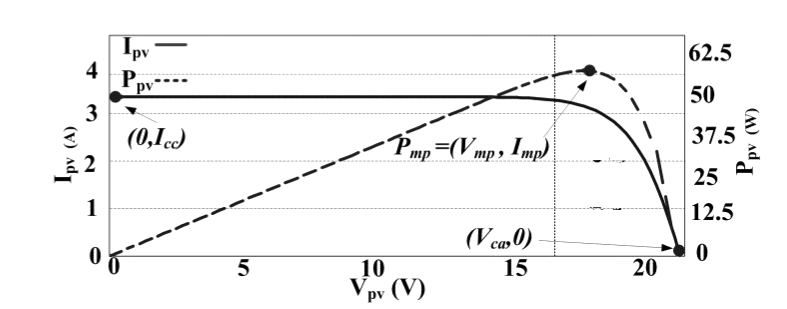
\includegraphics[scale = 0.25]{Figuras/Curva_MPPT.png}
            \caption{$I_{PV}$ y $P_{PV}$ vs $V_{PV}$ \cite{gallardo2014diseno}  }
            \label{fig: Curva MPPT}
        \end{figure}
    
    Existen diversas topologías para el conversor propuesto. En \cite{Kiran} se propone un conversor con un solo transistor y  de \textit{soft switching}, en \cite{9106477} un circuito de alta eficiencia, de diseño complejo por la cantidad de inductores; en \cite{5701795} se propone un conversor de topología convencional junto con su controlador analógico para una variación de entrada determinada; y en \cite{6119227} un conversor que combina topología KY y Buck para lograr un conversor estable. En \cite{954206} se puede observar comparaciones entre algunas topologías. En este trabajo se propone un conversor de simple implementación, bajo costo y eficiencia aceptable, con modo de funcionamiento de conducción continua, para ser controlado a través de un microcontrolador como se realiza en \cite{Chang}. De esta forma, en conjunto con sensores de corrientes y tensión, se podrá lograr un conversor y regulador para cargas variables, y configuraciones de paneles diferentes, configurables a través de una interfaz.
 
    EXPLICAR DIVISION DE TRABAJO 
 
\section{Diseño}
    
    Se propone un conversor de tipo SEPIC \textit{single-ended primary-inductor converter} ya que posee, entre otras ventajas, ausencia de inversión de polaridad en la salida, bajo rizado de la corriente de entrada \cite{alvarez2019caracterizacion} y la utilización de un solo transistor MOSFET que facilitará la implementación del controlador en trabajos futuros. El circuito es el de la figura \ref{fig: Circuito sepic}
    \begin{figure}
        \centering
      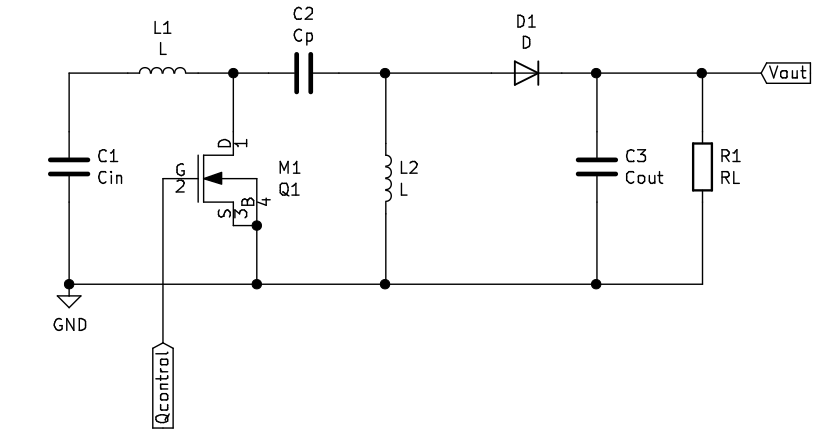
\includegraphics[scale = 0.25]{Figuras/Circuito_BB.png}
        \caption{Circuito sepic}
        \label{fig: Circuito sepic}
    \end{figure}
       
      
    En su mayoría, las diferentes topologías siguen un mismo procedimiento de diseño. Este trata de analizar al  conversor en sus dos modos de funcionamiento por separado, modo elevador y modo reductor de tensión. El diseño se realiza con este procedimiento mencionado, siguiendo lineamientos de \cite{espinosa2017asynchronous} y recomendaciones de notas de aplicación \cite{haifengdesign} y \cite{falin2008designing} considerando al conversor en modo de conducción continua (CCM). 
    
    Cuando el transistor Q1 se encuentra encendido (ON) 
    
    
    capacitor C P is charged to the input voltage,
V IN . Knowing this, we can easily determine
the voltages as shown in Figure 3.
When Q1 is off, the voltage across L1b
must be V OUT . Since C IN is charged to V IN ,
the voltage across Q1 when Q1 is off is V IN +
V OUT , so the voltage across L1a is V OUT . When
Q1 is on, capacitor C P , charged to V IN , is con-
nected in parallel with L1b, so the voltage
across L1b is –V IN .
    
    
    
       
      
  
    
    

\section{Resultados}
 
    Explico un poco qwue se obtuvo y meto algunas curvas 
    
    Este circuito será parte de un sistema complejo como el que puede verse en la figura ... 
    
Presenta una fácil implementación y
aislamiento galvánico entre la entrada y la salida, y un menor rizado de corriente
de entrada a altas frecuencias. Sin embargo, una mejora de este circuito puede
ser obtenida acoplando los dos inductores vistos bajo un mismo núcleo, teniendo
la posibilidad de aumentar la eficiencia en un 2 y reduciendo la emisión de ruido
EMI, lo que conlleva a simplificar el filtro de entrada del convertidor.\cite{rios2017sistema}
 
\section{Conclusión}

Trabajo a futuro. Diseño de convertidor multifase para mejorar la eficiencia. 
Eficiencia obtenida? 
Como se menicona en tal paper la eficiencia de este tipo podrìa ser mejorada, Ademas los componentes en modo boost sufren stress ... 




\nocite{*}
\bibliographystyle{plain}
\bibliography{Referencia/ref.bib}

\end{document}

